\documentclass[11pt]{article}
\usepackage[utf8]{inputenc}
\usepackage[main=french]{babel}
\usepackage{geometry}
\geometry{hmargin=2cm,vmargin=3.5cm}
\usepackage{graphicx}
\usepackage{amsfonts}
\usepackage{ulem}
\usepackage{amsmath}
\usepackage{esint}
\usepackage{calc}
\usepackage{array, multirow, makecell}
\usepackage{caption}
\usepackage{subcaption}
\usepackage{longtable}
\usepackage{multicol}
\usepackage{float}

\newcolumntype{R}[1]{>{\raggedleft\arraybackslash }b{#1}}
\newcolumntype{L}[1]{>{\raggedright\arraybackslash }b{#1}}
\newcolumntype{C}[1]{>{\centering\arraybackslash }b{#1}}

\title{\LARGE\textsc{{Génie Industriel}}}
\author{AlexCast}
\date{2019/2020}

\begin{document}

\begin{titlepage}
\begin{center}
    \vspace*{\stretch{1}}
$$   \begin{array}{cc}
        \mbox{\Huge\textsc{{Machine Learning}}}\\
        \mbox{Alexandre Castelnau}\\
        \mbox{Fall 2021}
    \end{array}$$
    \vspace*{\stretch{1}}
\end{center}
\begin{figure}[b]
    \centering
    
\includegraphics[width=10cm]{GT-logo.jpg}
\end{figure}
\end{titlepage}
\newpage

\tableofcontents
\newpage

\begin{multicols}{2}

\section{Definition of MDPs}

In this assignment, we will consider two MDPs in order to evaluate, test and understand the methods for solving the Bellman equation and the Reinforcement Learning techniques. 

Thus, in the next paragraphs, we will describe the two MDPs.

\subsection{Forest Management MDP}

The first problem is the management of a forest. It can be visualized as follows: in a given state of the forest, one can decide to cut the forest or to wait. In the first states of a forest, cutting it down brings only a small reward, heating with twigs. However, if we are in the later state, if we cut, we have good big logs (much better than twigs), but we can also make the choice not to touch the forest and be able to feed by making the biodiversity flourish (preferable choice). In all cases where one chooses to cut, the forest returns to its initial state. The action of waiting allows him to reach a new stage, but there is a probability $p$ that a fire comes to destroy all.

This rather simple model can be represented as follows:

\begin{figure}[H]
\centering
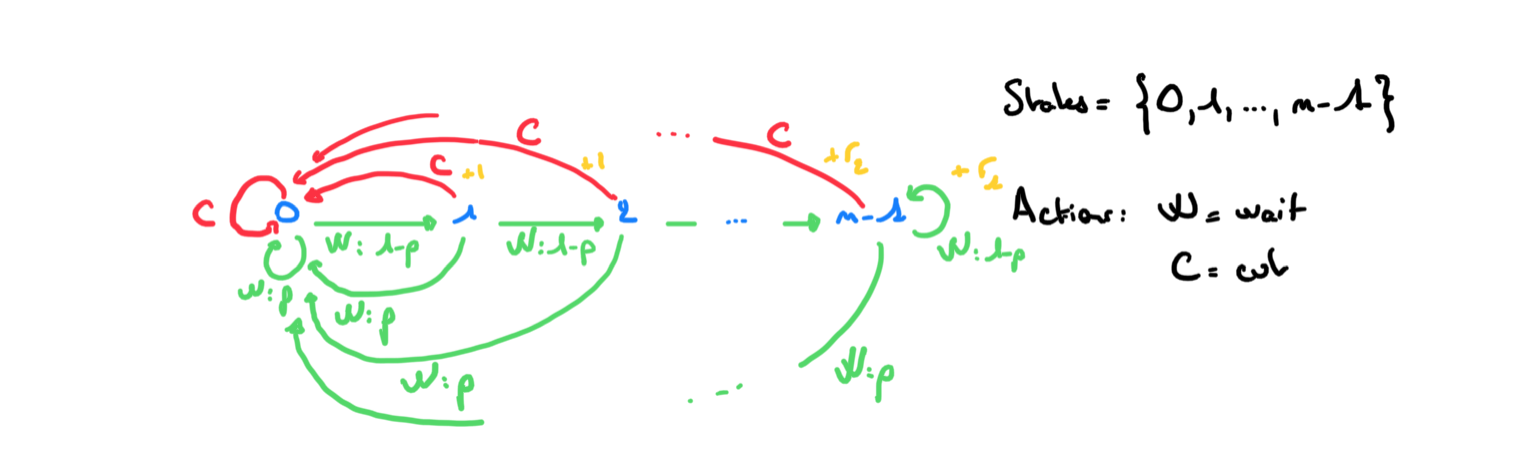
\includegraphics[width = \columnwidth]{mdp_fm.png}
\caption{Represention of the Forest Management MDP}
\end{figure}

With a more mathematical way, we can define the problem in such way:
\begin{itemize}
\item $n$ states: $\lbrace 0, 1, \dots , n-1 \rbrace$
\item $2$ actions: $0$ = Wait, $1$ = Cut
\item $2\times n \times n$ transition matrix where: 
$$P(0,:,:) = \left[\begin{array}{cccccc}
p & 1-p & 0 & \dots & \dots & 0 \\ 
\vdots & 0 & 1-p & 0 & \dots & 0 \\ 
\vdots & \vdots & 0 & \ddots & • & \vdots \\ 
\vdots & \vdots & \vdots & • & \ddots & 0 \\ 
\vdots & \vdots & \vdots & • & • & 1-p \\ 
p & 0 & 0 & \dots & 0 & 1-p
\end{array}\right]  $$
$$P(1,:,:) = \left[ \begin{array}{cccc}
1 & 0 & \dots & 0 \\ 
\vdots & \vdots & • & \vdots \\ 
\vdots & \vdots & • & \vdots \\ 
1 & 0 & \dots & 0
\end{array}  \right] $$
\item $n\times 2$ reward matrix:
$$ R = \left[\begin{array}{cc}
0 & 0 \\ 
\vdots & 1 \\ 
\vdots & \vdots \\ 
0 & 1 \\ 
r_1 & r_2
\end{array} \right] $$
\end{itemize}

This MDP will allow us to make an easily interpretable study of the methodologies. We can also play with the hyperparameters of the model to see their effects on the results. Moreover, as we can see, in this MDP we can easily choose to change the number of states, it can be interesting to use that fact to check the scalibility of our algorithms.

\subsection{Grid World-like MDP}

For the second problem, we assume we are living in a grid-like world. For that, I defined a $5\times 8$ grid with walls. The following figure shows the world I defined.

\begin{figure}[H]
\centering
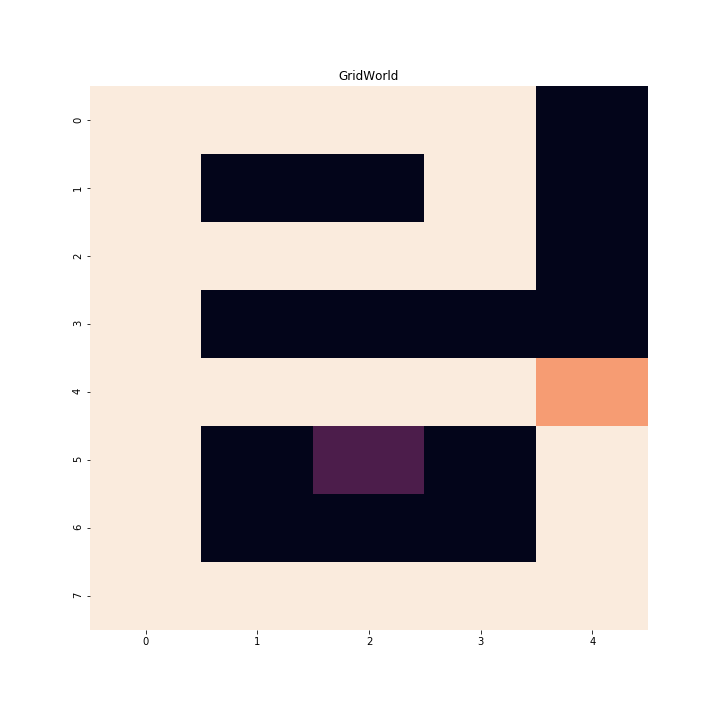
\includegraphics[width = \columnwidth]{gw.png}
\caption{Grid World}
\end{figure}

In this world, there is four possible action: Up, Down, Left, and Right. Meanwhile, when we choose to do one of the four previously mentionned actions, there is a slight chance we slide by side (stochastic world). The probabilities when we choose to go Up are:
\begin{itemize}
\item $0.8$ to go Up, what we wanted
\item $0.1$ to go Left
\item $0.1$ to go Right
\end{itemize}
The probabilities are expressed with the same logic for other actions. Also, because there is wall, if we go "inside" a wall, we just don't move. Moreover, in this world, I choose to define that each step will cost (energy consumed to move, $r_s = -1$) and there is a trap (for instance a hole with a "reward" $r_h$) and also a real reward $r_g =10$. I will not exhaustively express the transition and reward matrix, but their dimensions are respectively $4\times 40 \times 40$ and $40\times 40$. This MDP has the advantage to be simple and visual, it will be very useful to check the result of our algorithm (if the output seems to follow our intuition).

\section{Solving the Bellman equation: implementations of Policy Iteration and Value Iteration algorithms}

In the framework of these MDPs, we wish to determine the best policy to obtain the maximum reward (within the framework defined by the MDPs). We thus find ourselves in an optimization problem (we had seen in the assignment on Randomized Optimization that any problem could be translated into an optimization problem).

More particularly, we will consider two first algorithms that can allow us to solve the following problem (or at least a close approximation):

$$\text{Find } \pi^{*} = \underset{\pi}{\text{argmax}} \: \mathbb{E} \left[ \sum_t \gamma^t R(S_t) \; | \; \pi \right]$$

These two methods are : 
\begin{itemize}
\item Policy Iteration
\item Value iteration
\end{itemize}

The previous definition of our problem as "finding the policy with the highest reward expectancy" leads us to define the state's utility notion. It is simply what we can expect to win when we begin in this state:

$$ U^\pi(s)=\mathbb{E} \left[ \sum_t \gamma^t R(S_t) \; | \; \pi, \, s_0 = s \right]$$ 

\subsection{Value Iteration Algorithm}

\subsubsection{Description of the algorithm}
Let's start by analyzing the performance of the simplest algorithm, the Value Iteration Algorithm. This algorithm is a straightforward application for the search of the optimal state value function.

Let $U(s)$ be the "true" value of a state $s$. We have no prior knowledge of this value, so let $\hat{U}(s)$ be our approximation of the value.

We begin by "making a guess" (initialization step). Then we use an iterative process to converge close the optimal value by using the Bellman's equation:
$$\forall s \in S, \; \hat{U}_{t+1}(s) = R(s) + \gamma\, \underset{a}{\max} \sum_{s'} T(s, a, s')\hat{U}_t(s')$$
For a MDP with $n$ different states, we obtain a system of $n$ equations with $n$ unknown. It is a good thing, unfortunately it is not a set of linear equation, we can't use methods such as Gauss' pivot to quickly compute the answer. Hence, this algorithm can be time consuming.

Also, we let this algorithm runs to the convergence. We defined we reach the convergence when there is a iteration $T$ such as :
$$ \left| \hat{U}_T(s) - \hat{U}_{T-1}(s)  \right| < \epsilon$$
If we observe well the process we describe above, two important hyperparameters are used for this algorithm, $\gamma$ ($\approx$ learning rate) and $\epsilon$ ($\approx $ convergence), we will study how they can influence the algorithm performances.

\subsubsection{Applications}

For the forest management problem, we can observe for several tuples $(\gamma , \epsilon)$, the time speed of the algorithm, the number of iterations needed to reach convergence but also the evolution of $V_{max}$ and $V_{mean}$ on the problem with the largest number of states.

We can observe that there is a dependence between the execution time / number of iterations needed and the convergence criterion. Indeed, when we decrease the $\epsilon$ value, the algorithm becomes more demanding on the convergence and this requirement requires some additional iterations. However, the two characteristics just mentioned (time/iterations needed) depend much more on the hyperparameter gamma. Indeed, gamma is synonymous with our consideration. To have a reason for this relationship, it is enough to understand that anticipating a more distant future requires the consideration of more variables and thus requires more calculations. This is why in the case where $\gamma$ is $0.999$, the differences in iterations and time due to the values of epsilon are almost not perceptible anymore.

\begin{figure}[H]
\centering
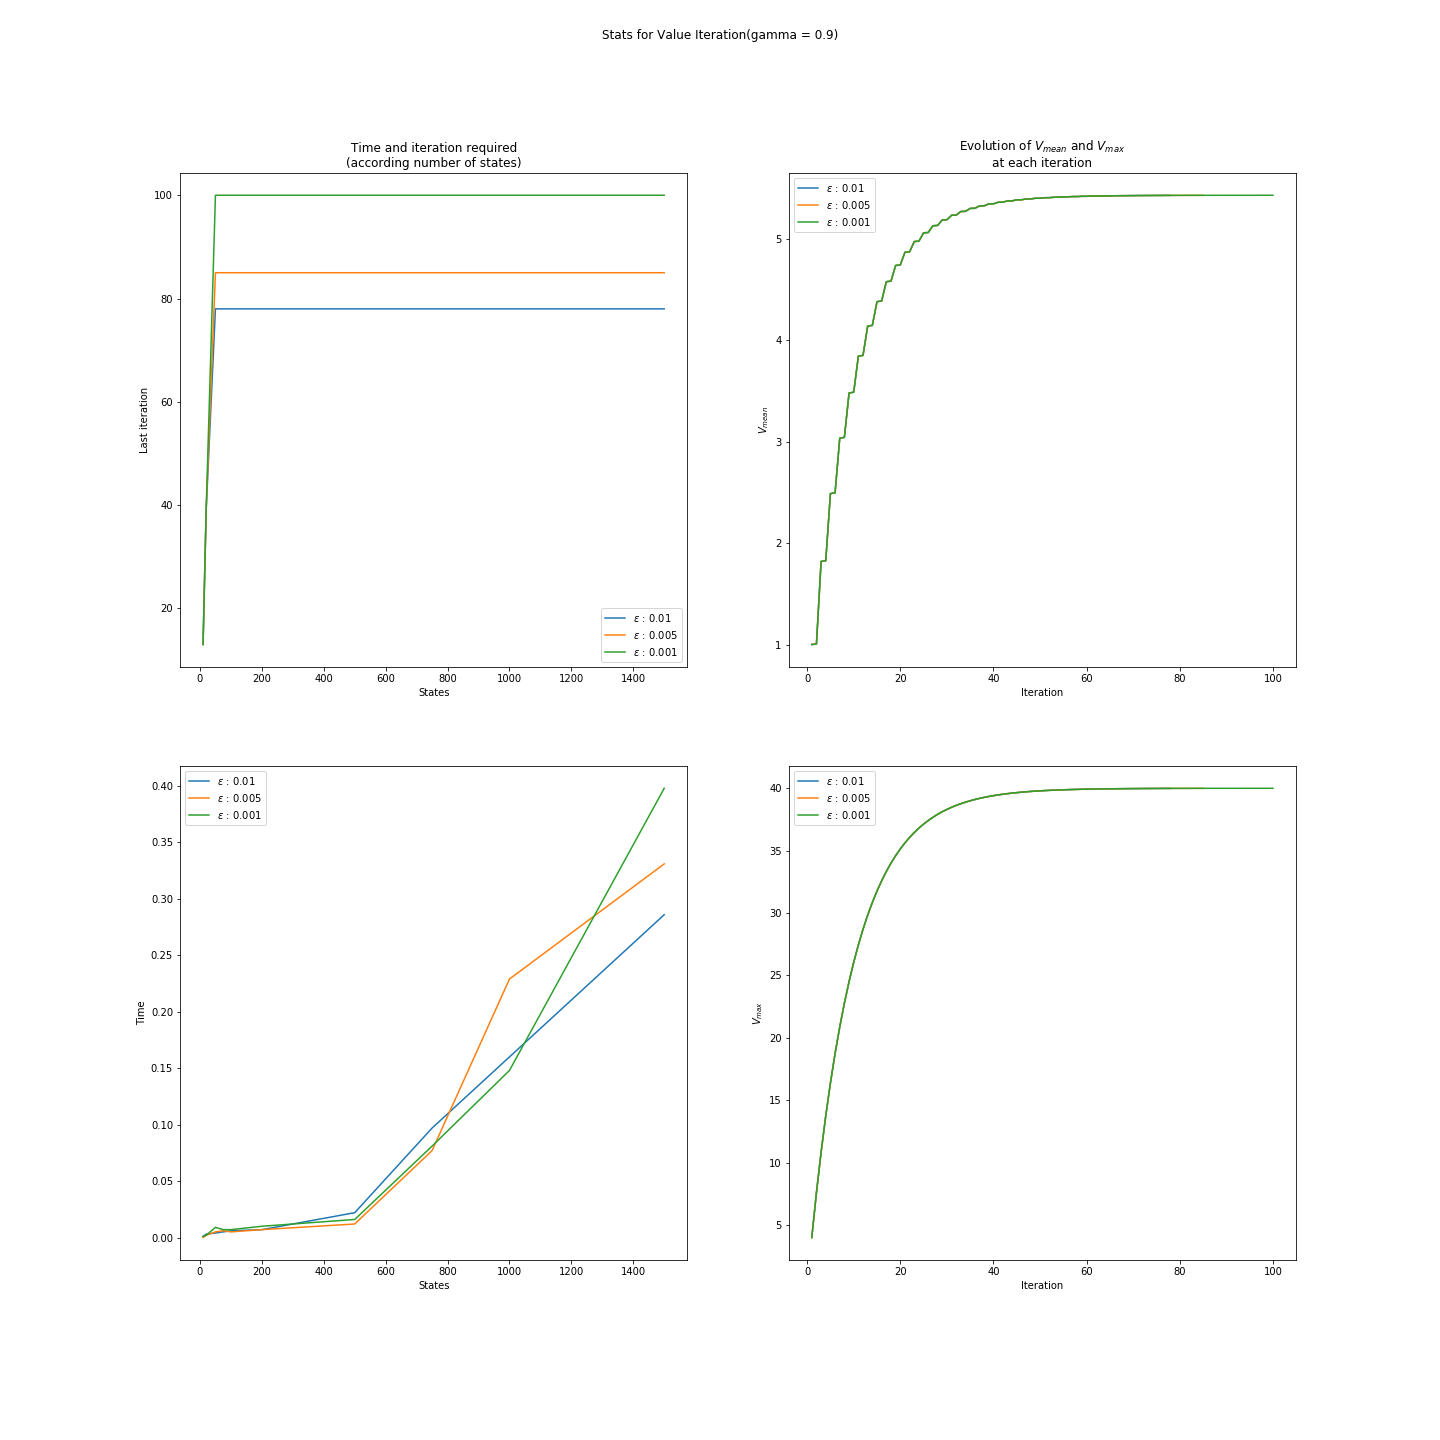
\includegraphics[width = 0.9\columnwidth]{VI_FM_0.9.png}
\caption{Performance of VIA (Forest Management, $\gamma = 0.9$}
\end{figure}

Finally, on the graphs on the right, we can observe the evolution of the values of $V_{max}$ and $V_{mean}$ during the iterations of the algorithm on the largest problem (1500 states). We immediately observe the superposition of the curves (whatever the $\alpha$ value). This is due to the deterministic character of the algorithm. For the same initialization, the step followed will be the same (no randomness in the process). The only difference that could be noted would be if the $\alpha$ values were too different, some curves would not go as far as the others (because they would have converged before the others).

For the Grid World problem, I plotted the same kind of graph and the conclusions are still the same. The algorithm will always converge towars the same values, if we get different answers (i.e. policies), it is just because we set the converge criterion quite differently.

\begin{figure}[H]
\centering
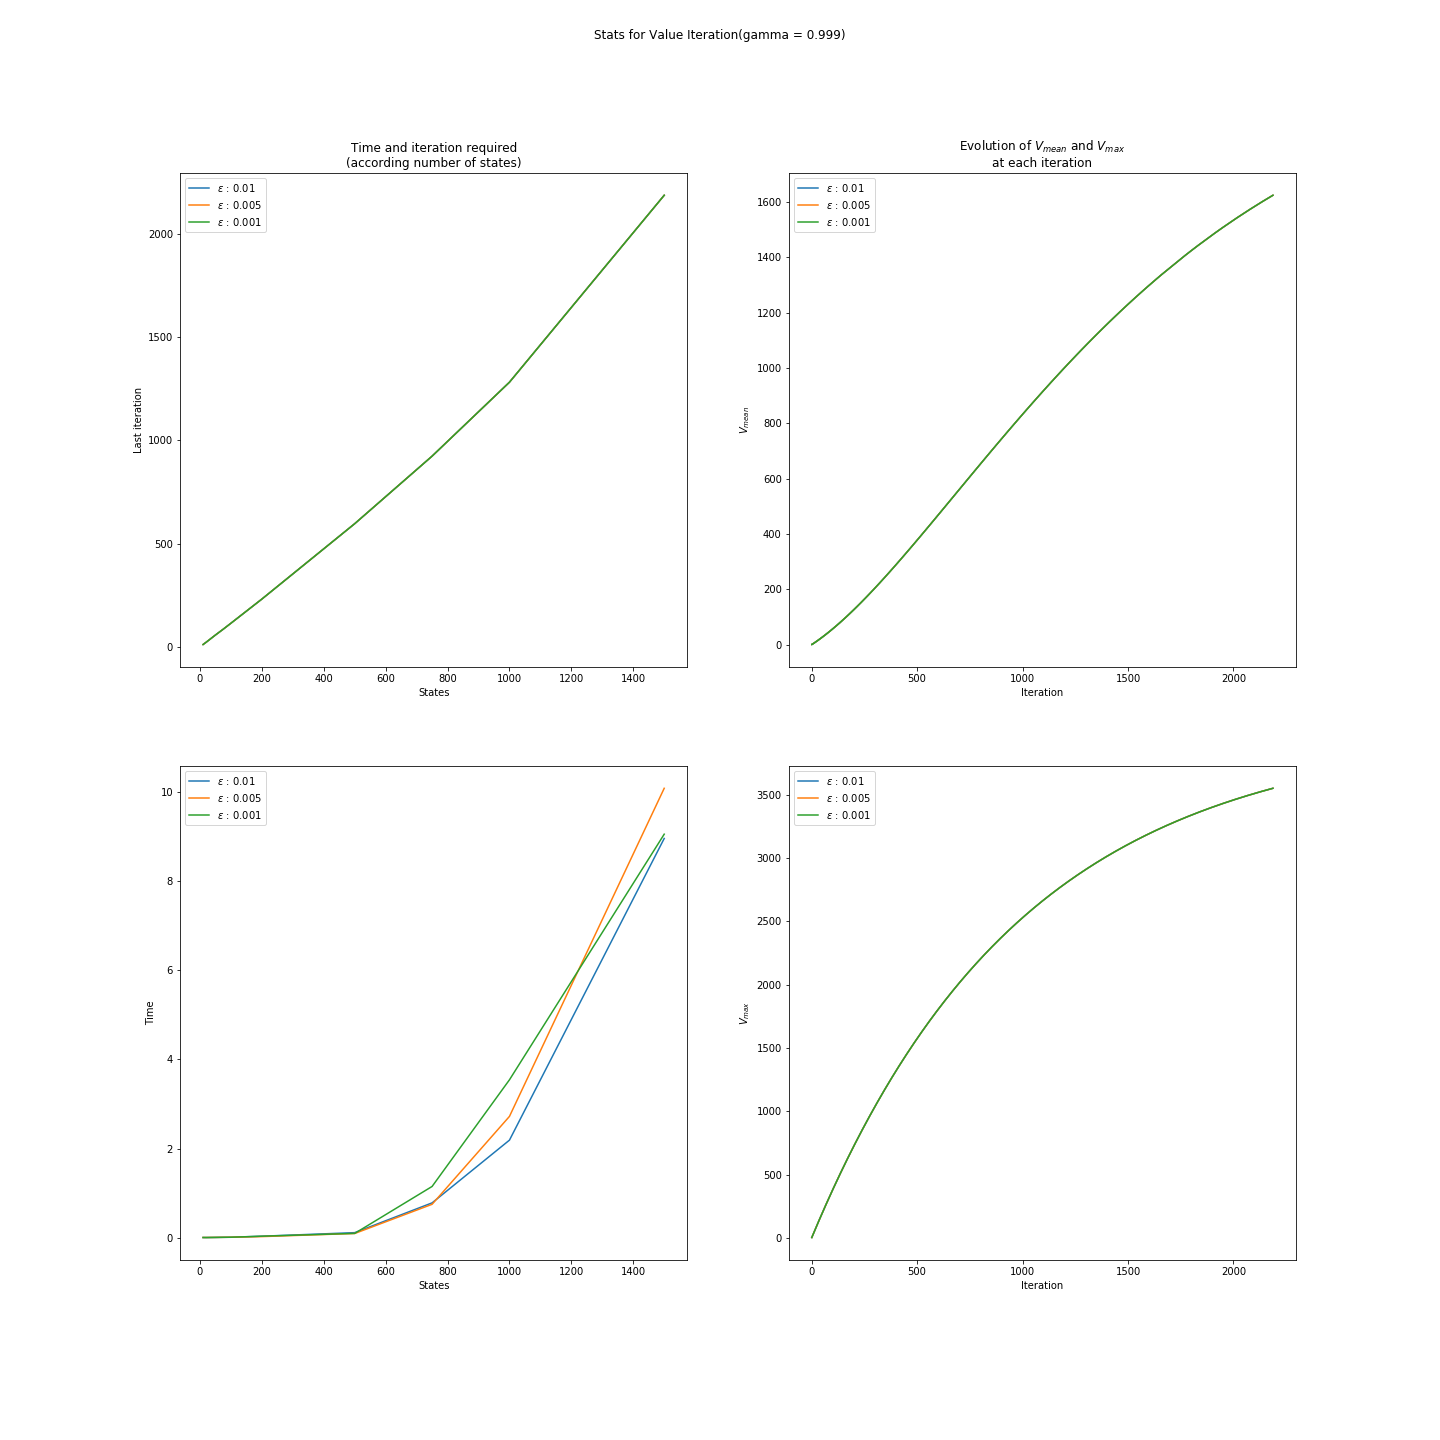
\includegraphics[width = 0.9\columnwidth]{VI_FM_0.999.png}
\caption{Performance of VIA (Forest Management, $\gamma = 0.999$}
\end{figure}

\begin{figure}[H]
\centering
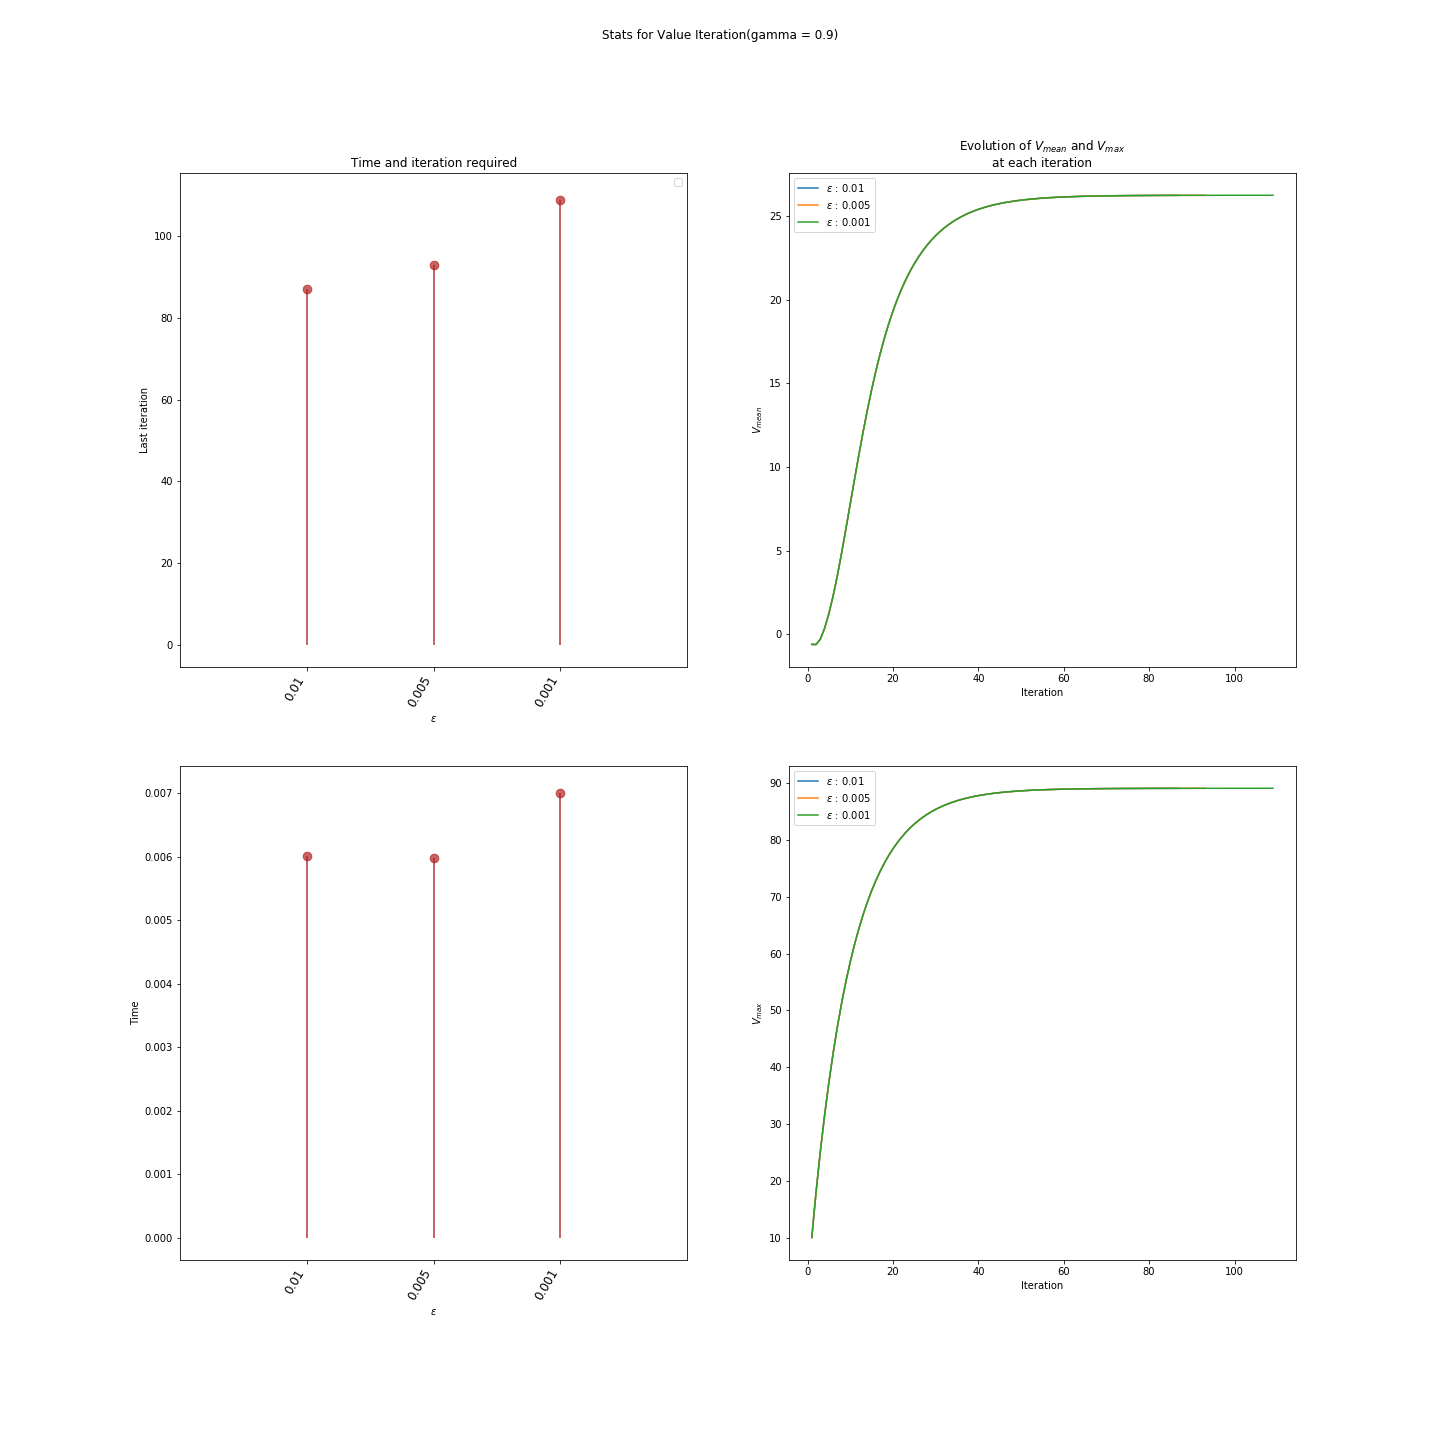
\includegraphics[width = 0.9\columnwidth]{VI_GW_0.9.png}
\caption{Performance of VIA (Grid World, $\gamma = 0.9$}
\end{figure}

\begin{figure}[H]
\centering
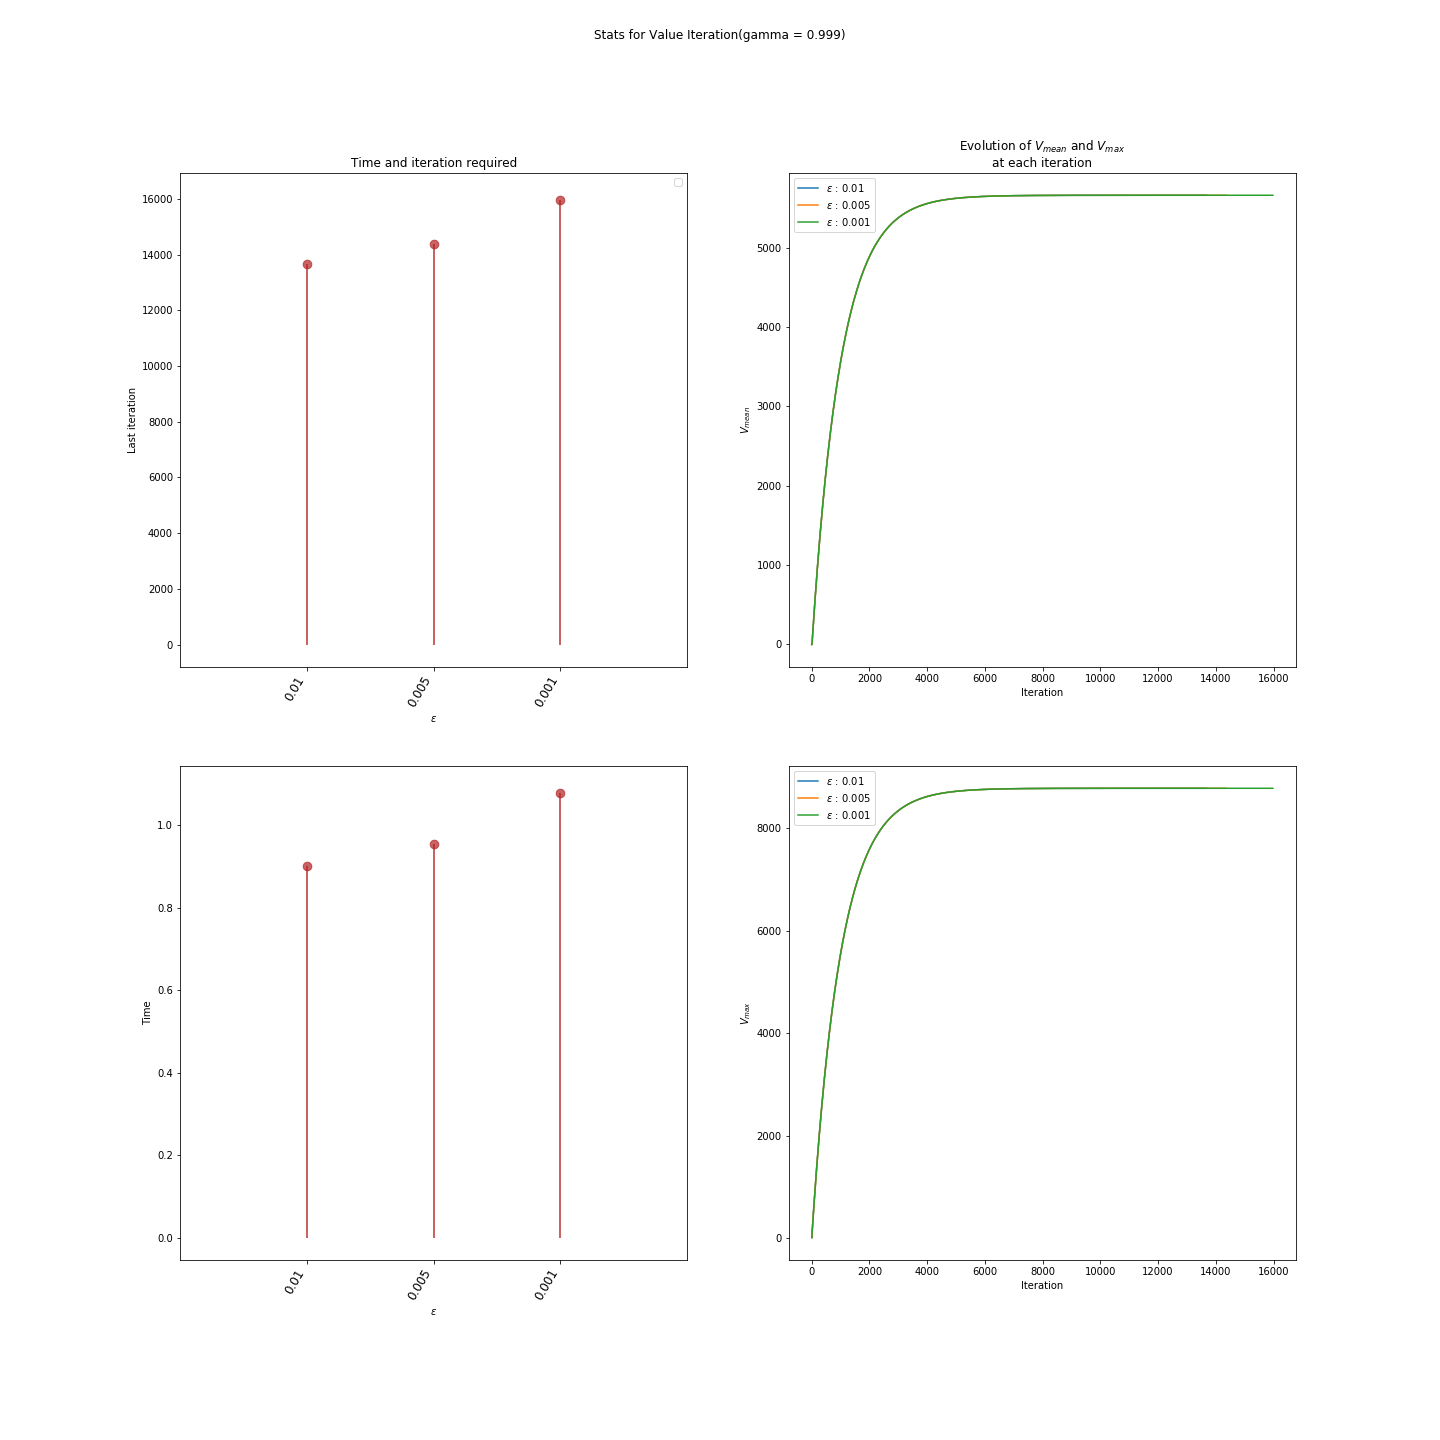
\includegraphics[width = 0.9\columnwidth]{VI_GW_0.999.png}
\caption{Performance of VIA (Grid World, $\gamma = 0.999$}
\end{figure}



\subsection{Policy Iteration Algorithm}

\subsubsection{Description of the algorithm}
After the straightforward Value Iteration Algorithm, we can use another similar method to obtain the optimal policy, the Policy Iteration Algorithm.

This algorithm is a little bit more complex than the previous one but is always profoundly tied the Bellman's equation. Its steps are the following:
\begin{itemize}
\item Initialization: Set the policy with a randomly chosen one $\pi = \pi_0$
\item Evaluation step: Compute $\hat{U}_t = U^\pi$
\item Improvement step: Find $\pi_{t+1}$ such as:
$$\pi_{t+1} = \underset{a}{\text{argmax}} \sum T(s, a, s') \hat{U}_t(s)$$
where the part is in fact equal to a linear version of the Bellman's equation:
$$\hat{U}_{t}(s) = R(s) + \gamma\,  \sum_{s'} T(s, a, s')\hat{U}_t(s')$$
\end{itemize}
We can observe that even if this algorithm seems to be slightly more complex, it is based on evaluation and sets of linear equations. If we are right, this method should be faster in term of iterations and time needed (we will check that later).

\subsubsection{Applications}

For this second algorithm, I proceeded with the study methodology. We can still observe the same relations between $\gamma$ and the execution time / number of iterations.

However, we can notice something very intriguing and that I cannot explain. It appears that when faced with similar problems, the "superiority" of the Policy Iteration Algorithm is not so true. Indeed, even if the number of iterations necessary to reach convergence is a little lower in all the problems treated, it appears that it is less performing in terms of temporal performance on the Forest Management Problem.

It is possible that this is due to the problem we are treating. Indeed, if we observe the definition of this problem, we quickly observe that we are facing a transition matrix with a majority of coefficients. Even if this does not influence the Policy Iteration Algorithm, it could be that it allows the Value Iteration Algorithm to do the maximum search step in a much shorter time than one would think and thus to compete in terms of time with this second algorithm.

Nevertheless, on the Grid World Problem, we can see the improvement that this second algorithm proposes compared to the first one because it allows to obtain a result in a time almost 100 times lower.

Thus, I would be tempted to say that this second algorithm seems, as we thought at the beginning, more efficient on the majority of the problems we would face. However, in the case of problems with mainly empty transition matrices, the Value Iteration can be interesting. In any case, if we define the convergence in a well thought way, the two algorithms seem to converge to the same answer.

Moreover, even if it is not explicitly stated above, the number of states has a huge influence on the performance of the algorithms. It is even the main criterion to justify the variation in time...

\begin{figure}[H]
\centering
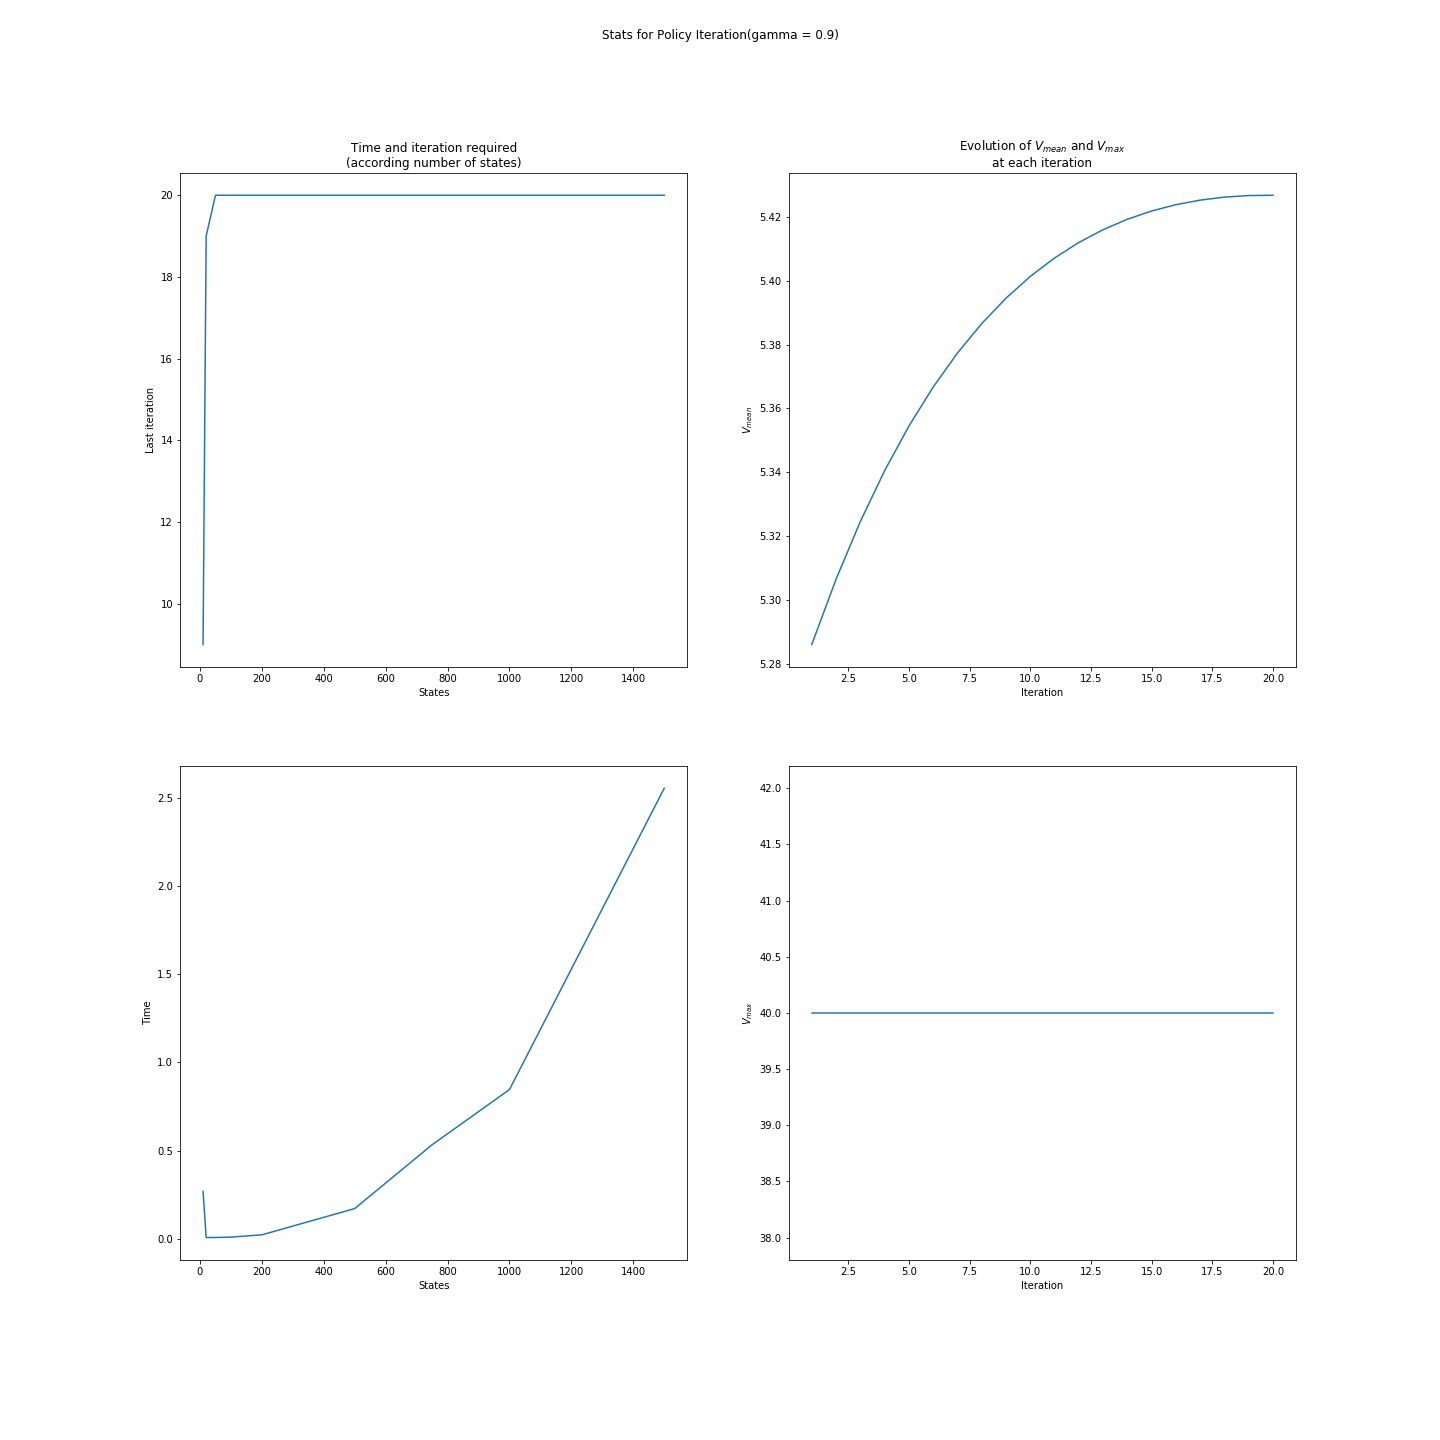
\includegraphics[width = 0.9\columnwidth]{PI_FM_0.9.png}
\caption{Performance of PIA (Forest Management, $\gamma = 0.9$}
\end{figure}


\begin{figure}[H]
\centering
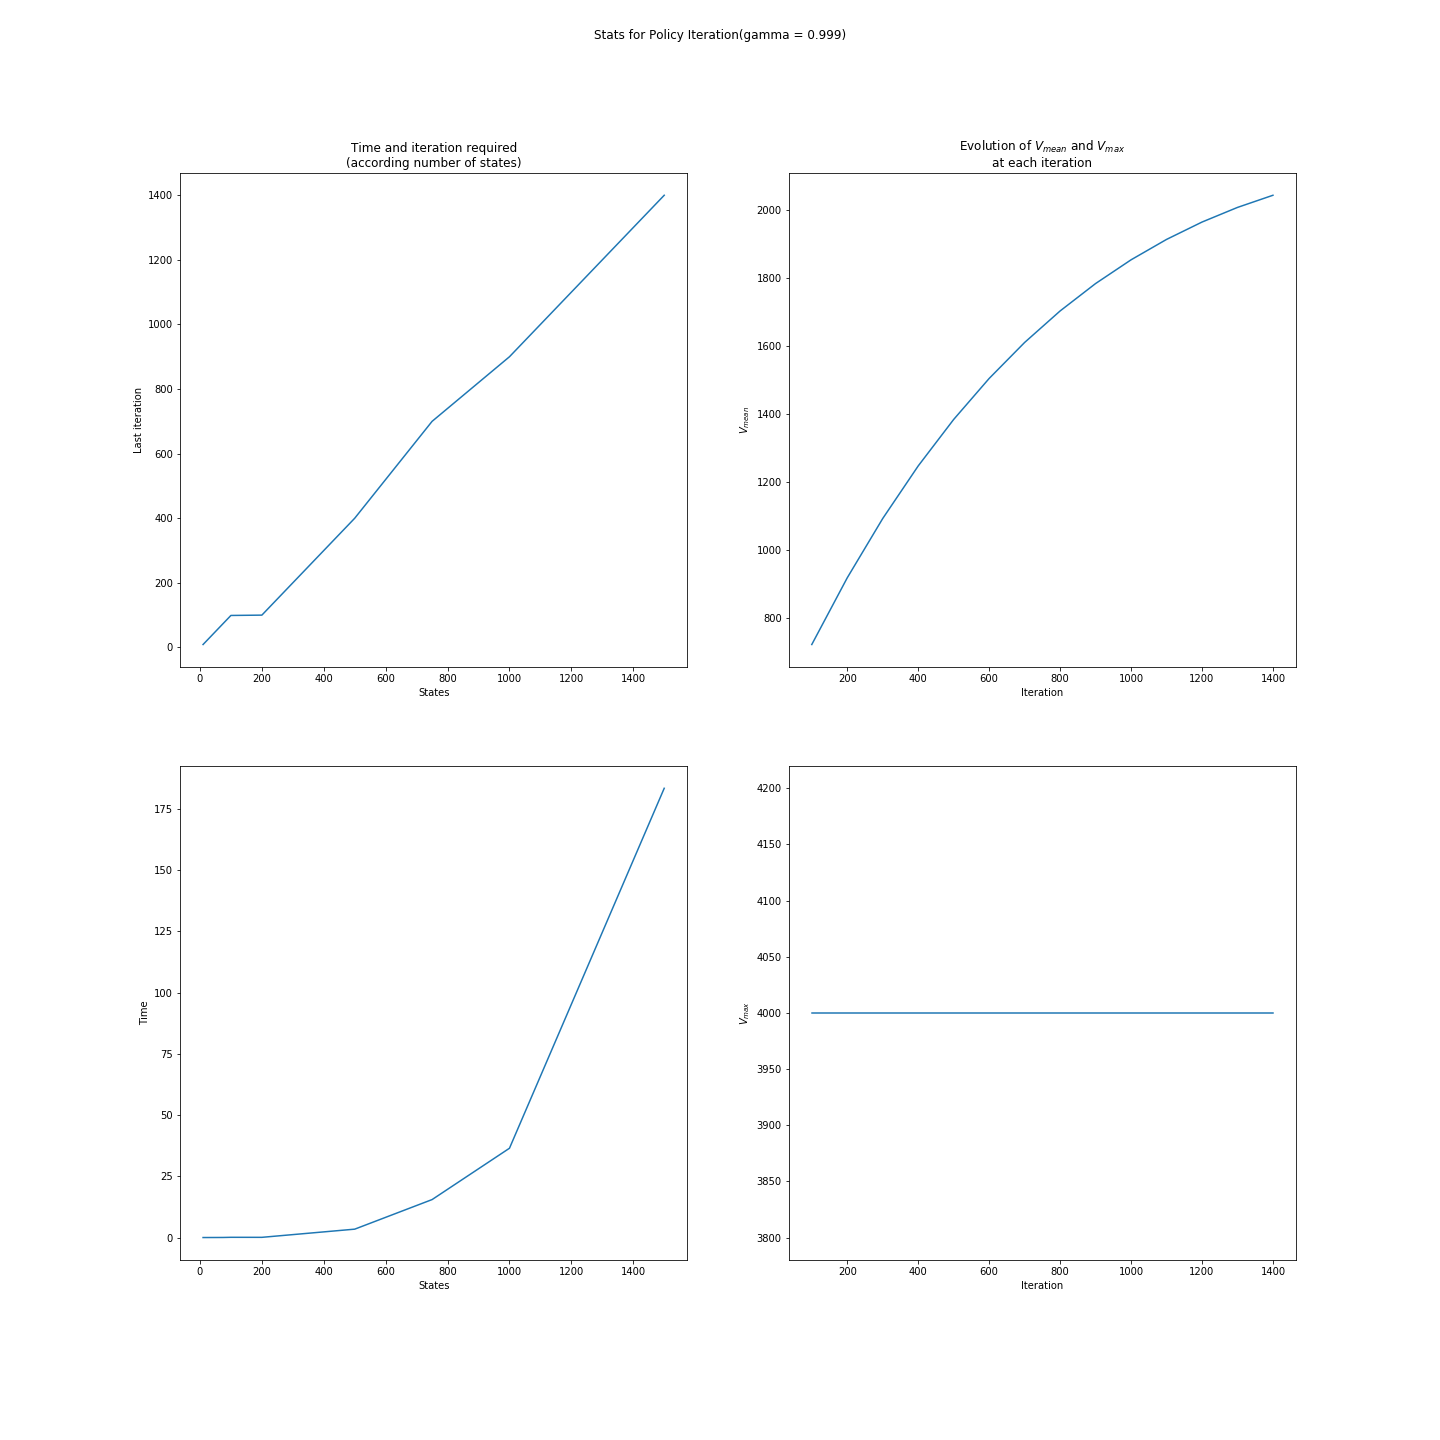
\includegraphics[width = 0.9\columnwidth]{PI_FM_0.999.png}
\caption{Performance of PIA (Forest Management, $\gamma = 0.999$}
\end{figure}

\begin{figure}[H]
\centering
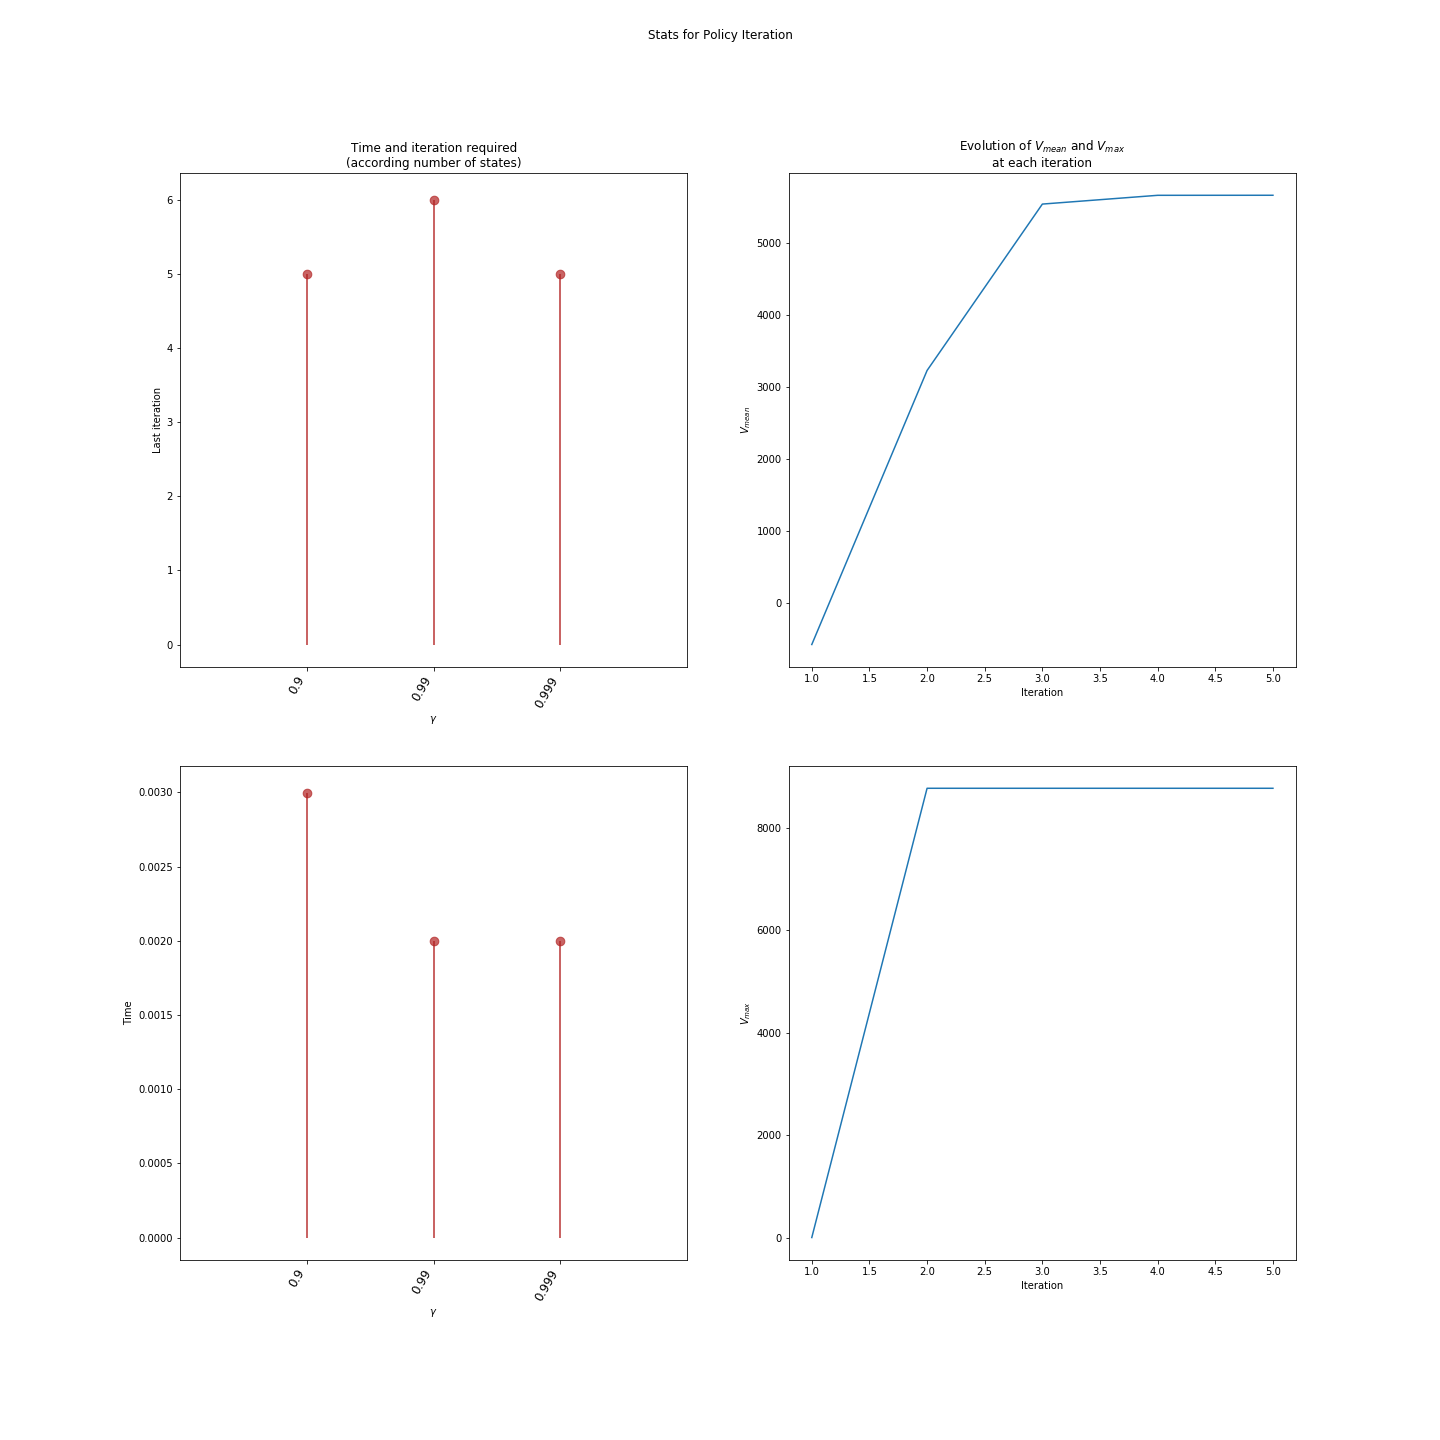
\includegraphics[width = 0.9\columnwidth]{PI_GW.png}
\caption{Performance of PIA (Grid World}
\end{figure}

\subsection{Influence due to the definition of the MDPs}

We have seen that differences in the performance of the algorithms and their response can be due to the hyperparameters that are chosen. However, even if we will not dwell too much on the subject (because it does not seem to be the goal here), but it is good to remember the importance of knowing how to correctly model a CDM if we are inspired by the real world. Indeed, the results can/will differ enormously depending on the way the problem is modeled.

\begin{figure}[H]
\centering
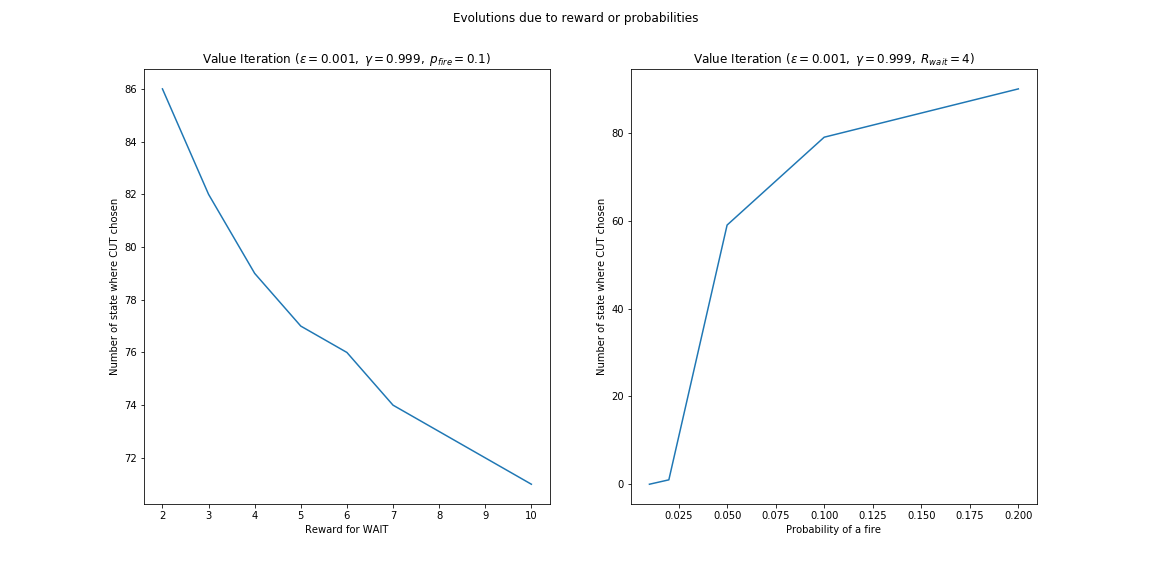
\includegraphics[width =  0.9\columnwidth]{Influence_rew_pb.png}
\caption{Influence due to variation in fire probability or reward}
\end{figure}

In the case of forest management, one will more easily opt to preserve it if one knows that the probability of a fire and/or the reward for preserving it is important.

In the case of the Grid World problem, if one assigns a high severity of falling into the hole, one will get a more conservative policy (which will induce one to make the detour to get the reward).

\begin{figure}[H]
\centering
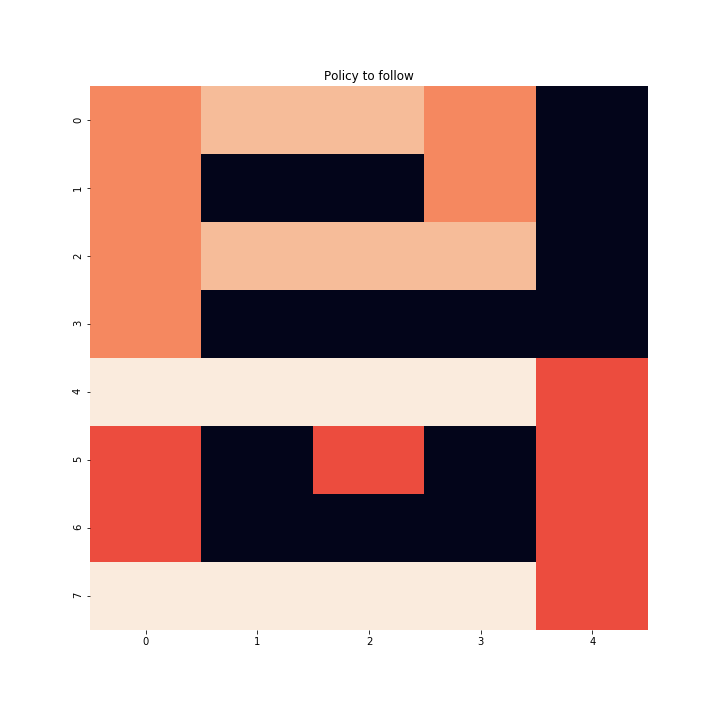
\includegraphics[scale =  0.2]{Policy_gw_10.png}
\caption{Policy obtained for small value of trap $r_s = -10$}
\end{figure}

\begin{figure}[H]
\centering
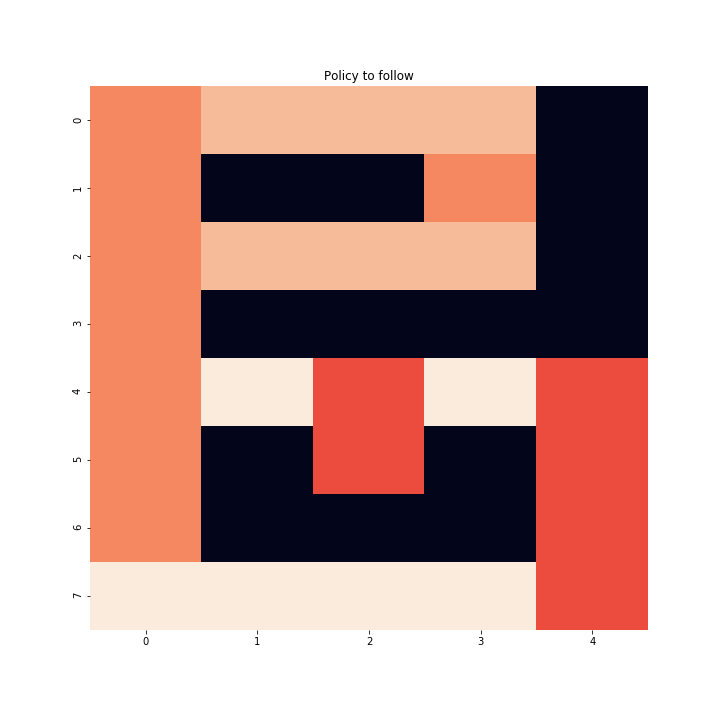
\includegraphics[scale =  0.2]{Policy_gw_1000.png}
\caption{Policy obtained for huge value of trap $r_s = -1000$}
\end{figure}

From the lightest color to the more reddish: Right, Left, Down, Up.

\section{Reinforcement learning applied to MDPs}

Before trying to explaining how we used Reinforcement Learning methods to MDPs, let's define what we will call the "quality" of a tuple state/action. This quality is defined this way: 
$$Q(s,a) = R(s) + \gamma \sum_{s'} T(s, a, s') \underset{a'}{\max} Q(s', a')$$

\subsection{Description of Q-Learning}

As we mentioned earlier, the problem we are facing seems similar to an optimization problem, why not take inspiration from the Randomized Optimization methods we saw earlier in the course in this new context?
An application of a modified version of Simulated Annealing seems to be a good idea, it is simple, rather efficient and allows to extract local optima. Let's remember how is defined this last \textit{SA}'s characteristic. 

We define for \textit{SA} a probability of "going back" according to the value of the neighbor, we are not always digging to find the best in the neighborhood. In \textit{SA}, this probability is parameterized (in other) by the initial value of the temperature (but slowly decreases). For instance, for an geometrical decay, this probability is defined at the time $t$ as:
$$ \mathbb{P} = \min \left(1, \exp (- \frac{F(y)-F(y)}{T(t)})\right)$$
where $x$ is the current state, $y$ is the neighbor and $T(t)$ the temperature at the time $t$. Hence, the probability of considering a neighbor with a lower value is all the more important as the initial temperature is large. 

Now, we can apply a similar method to find the best policy. The algorithm we get is the Q-Learning Algorithm, its steps are the following: 
\begin{itemize}
\item Initialization: Creation of a Quality table (the Q came from here) and we assign to this table only null values.
\item Action step: Exploring or Exploiting
\item Updating Q table
\end{itemize}

To spend a little more time about the   "Action Step", let explain what we think when we say "Exploring or Exploiting". We define an exploring probability  $\epsilon$ (and so, $(1-\epsilon)$ to exploite). Hence, sometimes the algorithm will not make a step toward the local optimum but will choose a random neighbor. It allows the algorithm to escape from a local optimum. We can see that the hyperparameter $\epsilon$ have a similar role than the \textit{SA} temperature. 

For the update, it is done following this rule:
$$ \hat{Q}(s, a) = (1-\alpha )\hat{Q}(s, a) + \alpha \left( R(s)+\gamma \underset{a'}{\max} \hat{Q}(s', a')  \right)$$
The hyperparameter $\alpha$ is the learning rate, while $\gamma$ correspond to the importance we give to "the future".


\subsection{Applications}

During my implementation of this algorithm, I was able to highlight the importance of the hyperparameter that we set for the maximum number of possible iterations. It is actually the main responsible for the performance of the algorithm. Indeed, it is with this last one that we fix the resources (temporal and computational) that we attribute to the algorithm to provide us an answer.

Also we observe naturally, that with high $\gamma$ values, we will need more iterations to converge to the optimal policy.

Also, contrary to the algorithms mentioned earlier (Value Iteration and Policy Iteration), we are dealing with a non-deterministic algorithm (randomness in the Exploration/Exploitation stage). Thus, when the algorithm is applied several times, the result may differ: 
\begin{itemize}
\item because it followed different paths and we cut the process with the limitation of iterations
\item or because by following different paths it finally got stuck in a local minimal.
\end{itemize}


\begin{figure}[H]
\centering
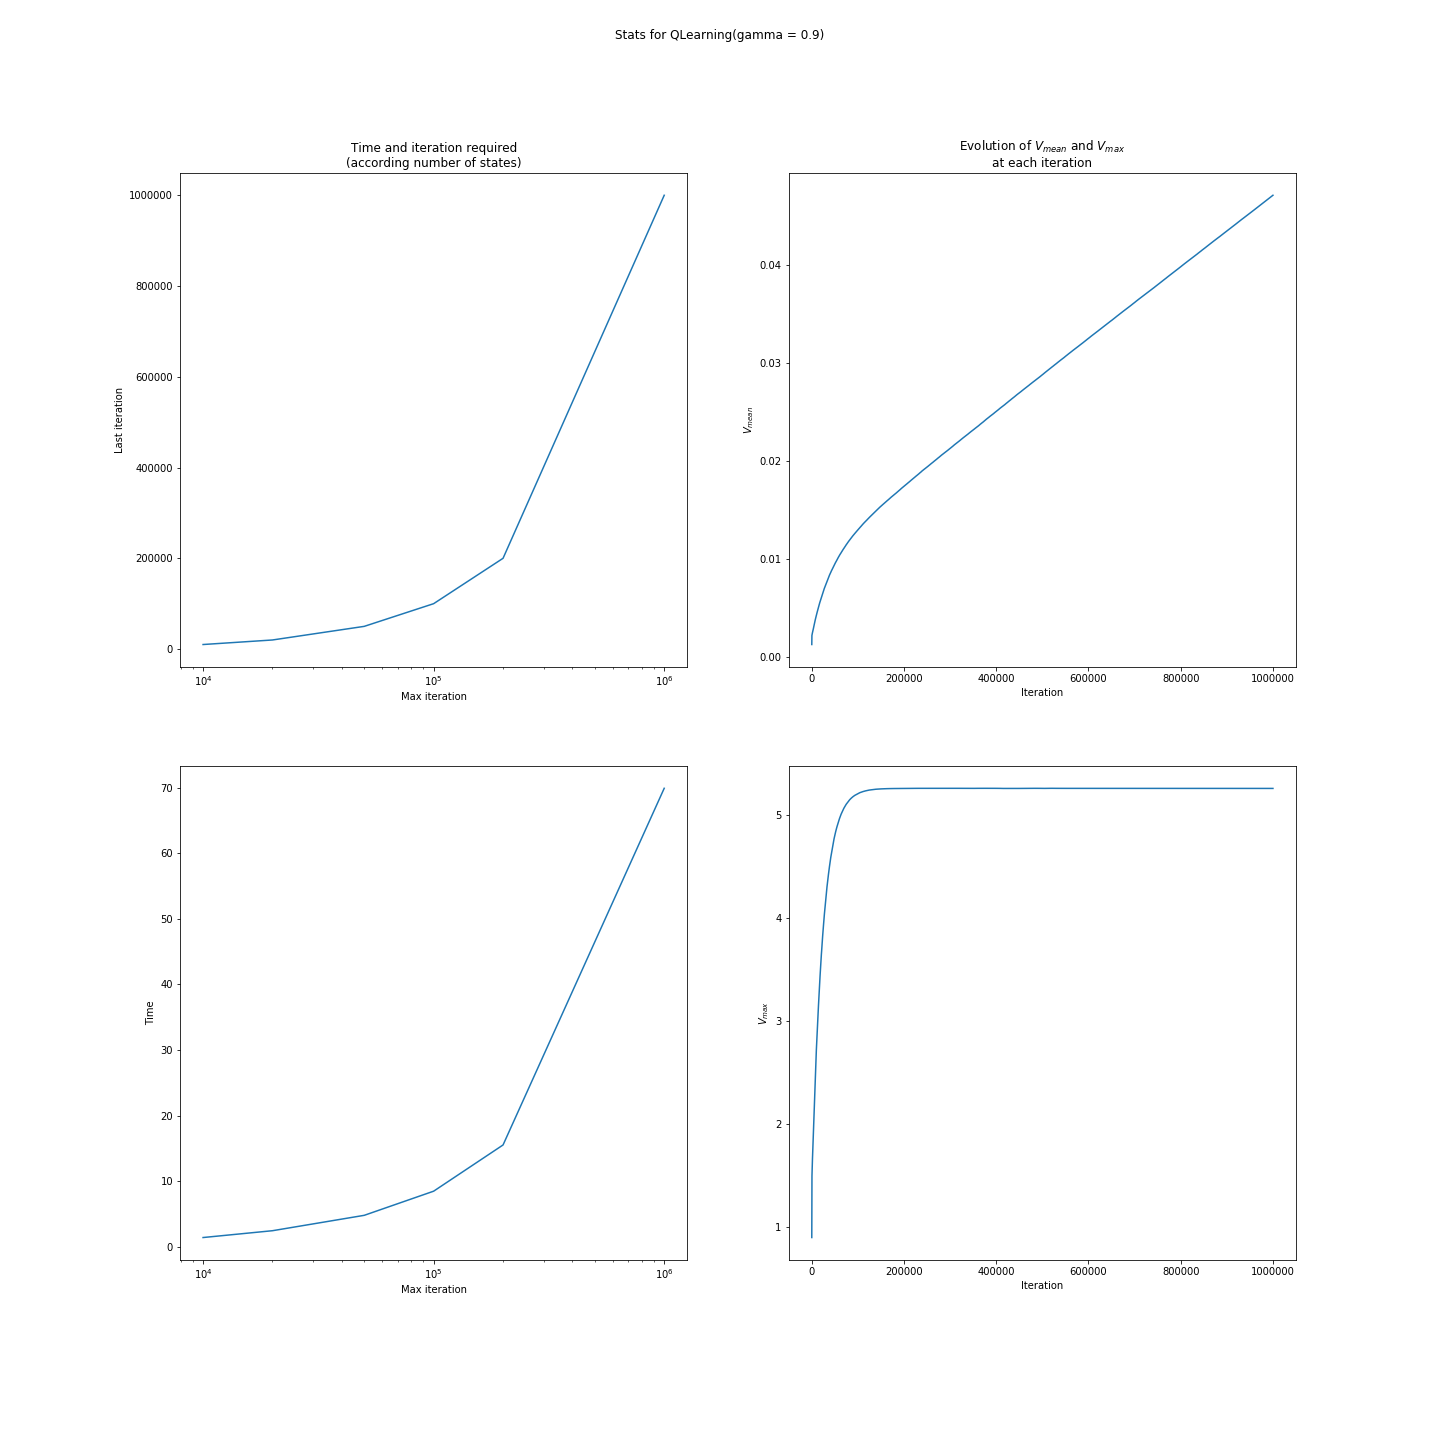
\includegraphics[width = \columnwidth]{Q_FM_0.9.png}
\caption{Evolution during the iterations ($\gamma = 0.9$)}
\end{figure}

\begin{figure}[H]
\centering
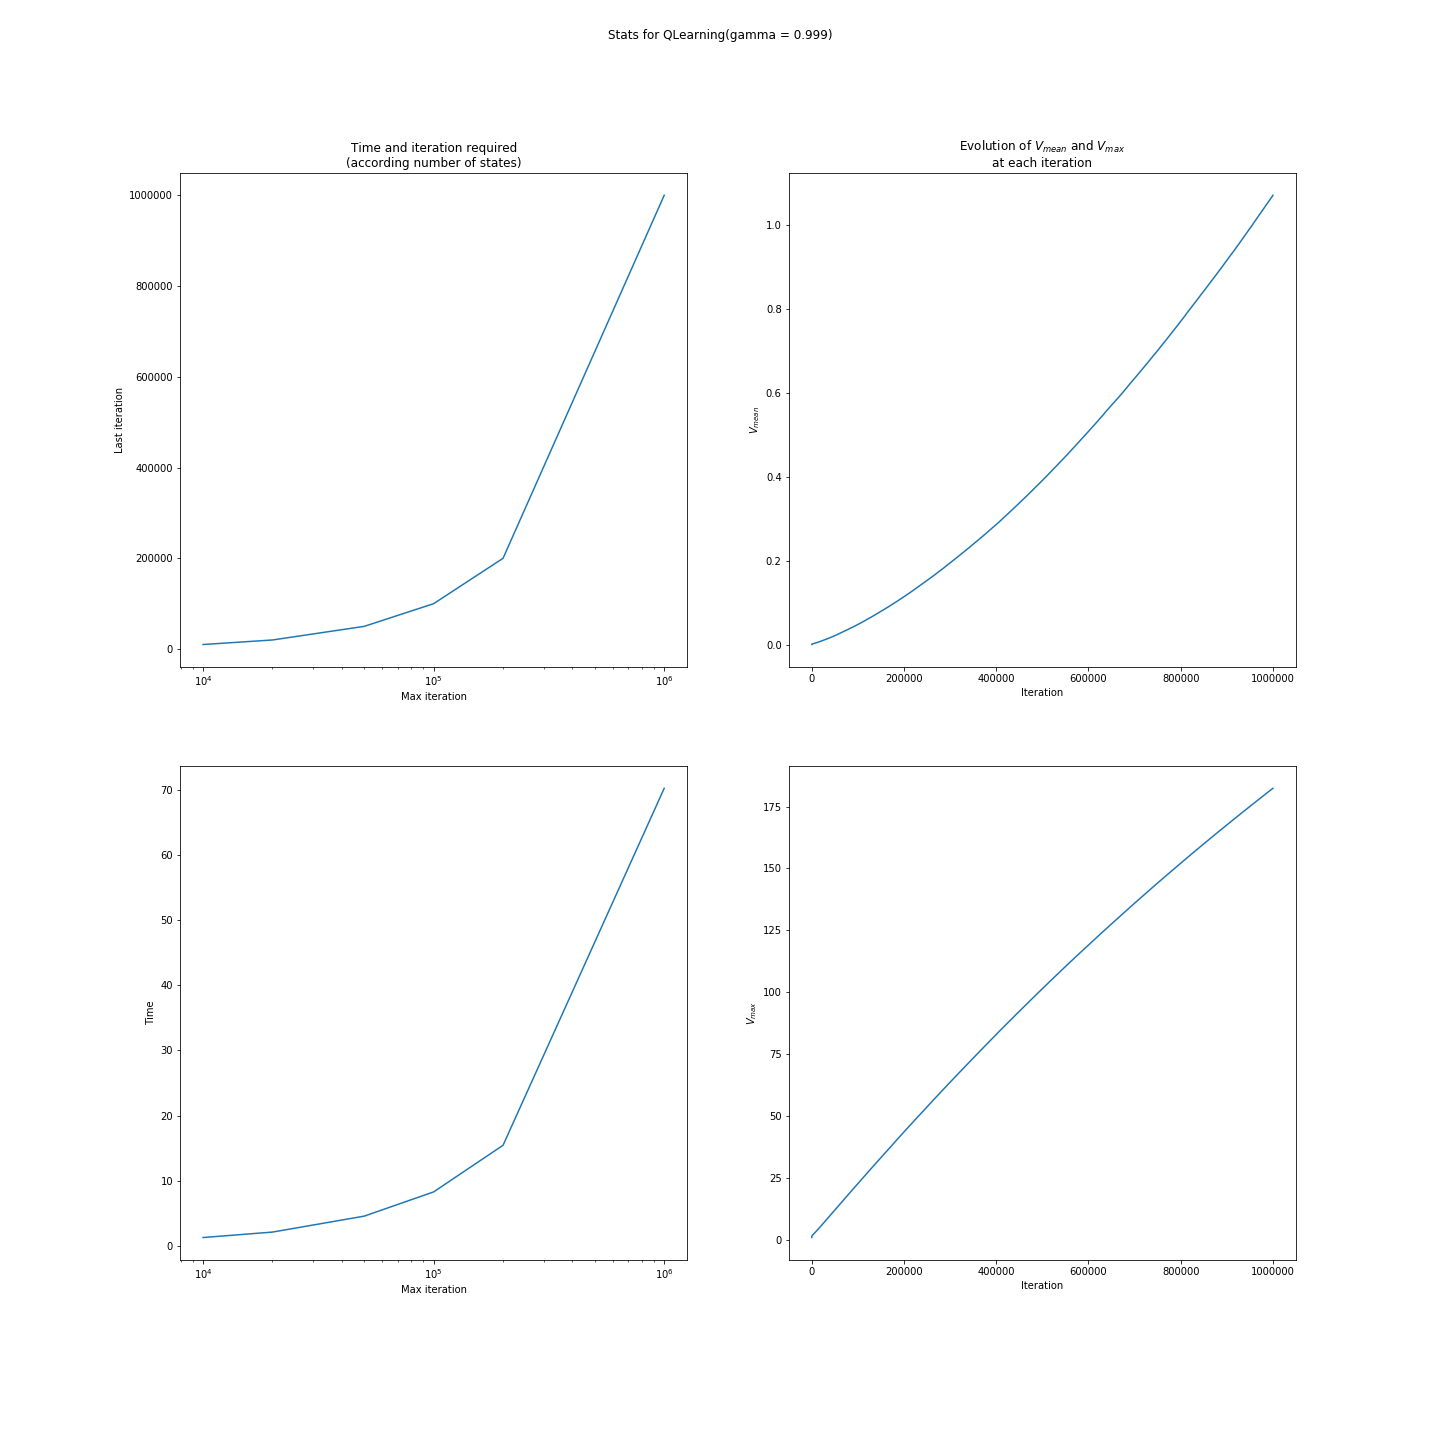
\includegraphics[width = \columnwidth]{Q_FM_0.999.png}
\caption{Evolution during the iterations ($\gamma = 0.999$)}
\end{figure}

Like for the SA, one can try to observe the effect of hyperparameters on the results of the algorithm. This is why I explored the potential influence of the hyperparameters $\epsilon$, $\alpha$ and their respective decay for the Grid World problem. Indeed, these hyperparameters told us the choice we made in the tradeoff between exploration and exploitation.

\begin{figure}[H]
\centering
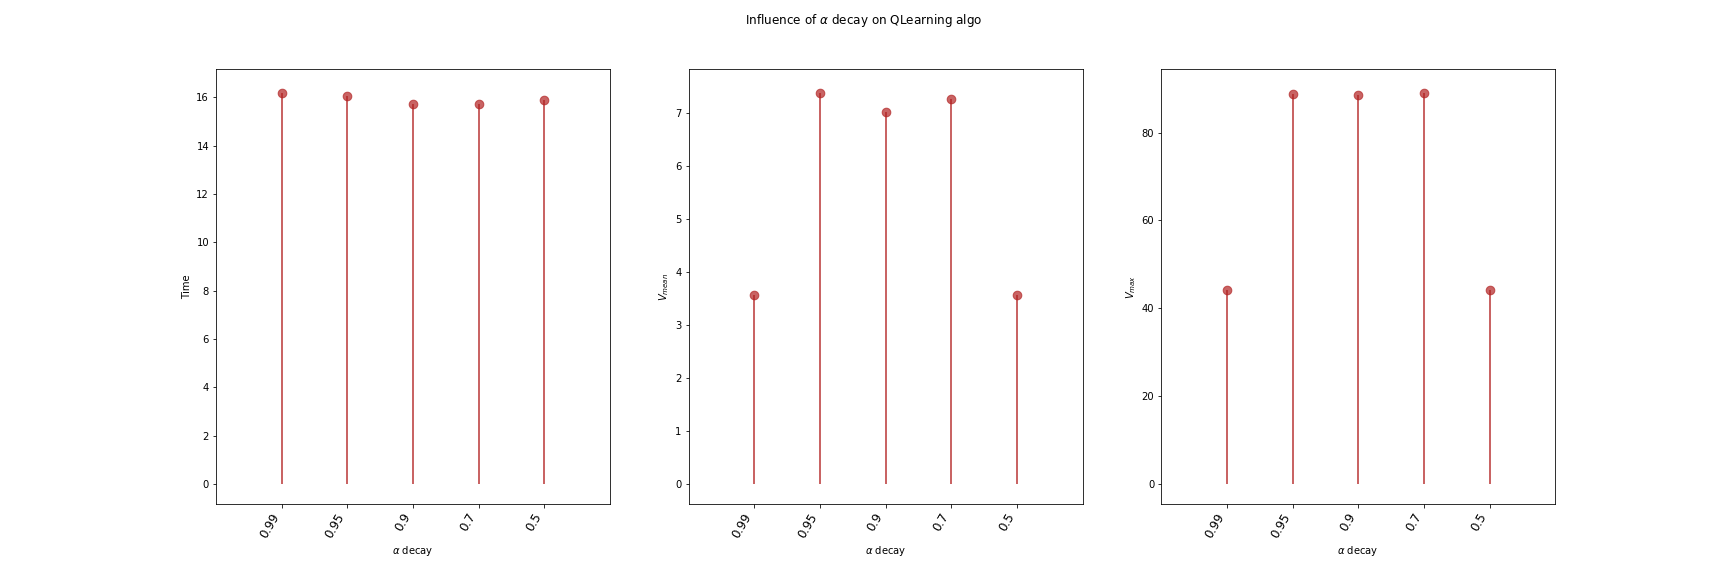
\includegraphics[width = \columnwidth]{aldec_ql.png}
\caption{Influence of $\alpha$ decay}
\end{figure}

\begin{figure}[H]
\centering
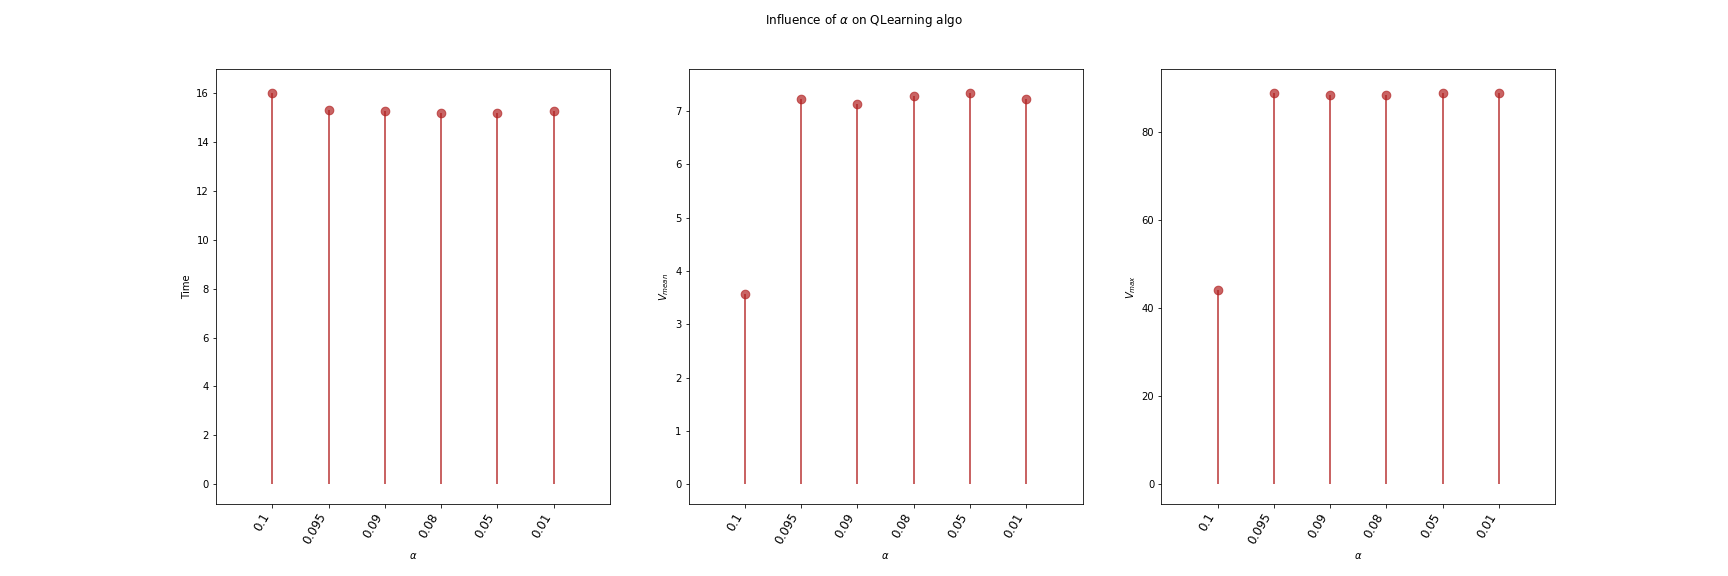
\includegraphics[width = \columnwidth]{alp_ql.png}
\caption{Influence of $\alpha_0$}
\end{figure}

\begin{figure}[H]
\centering
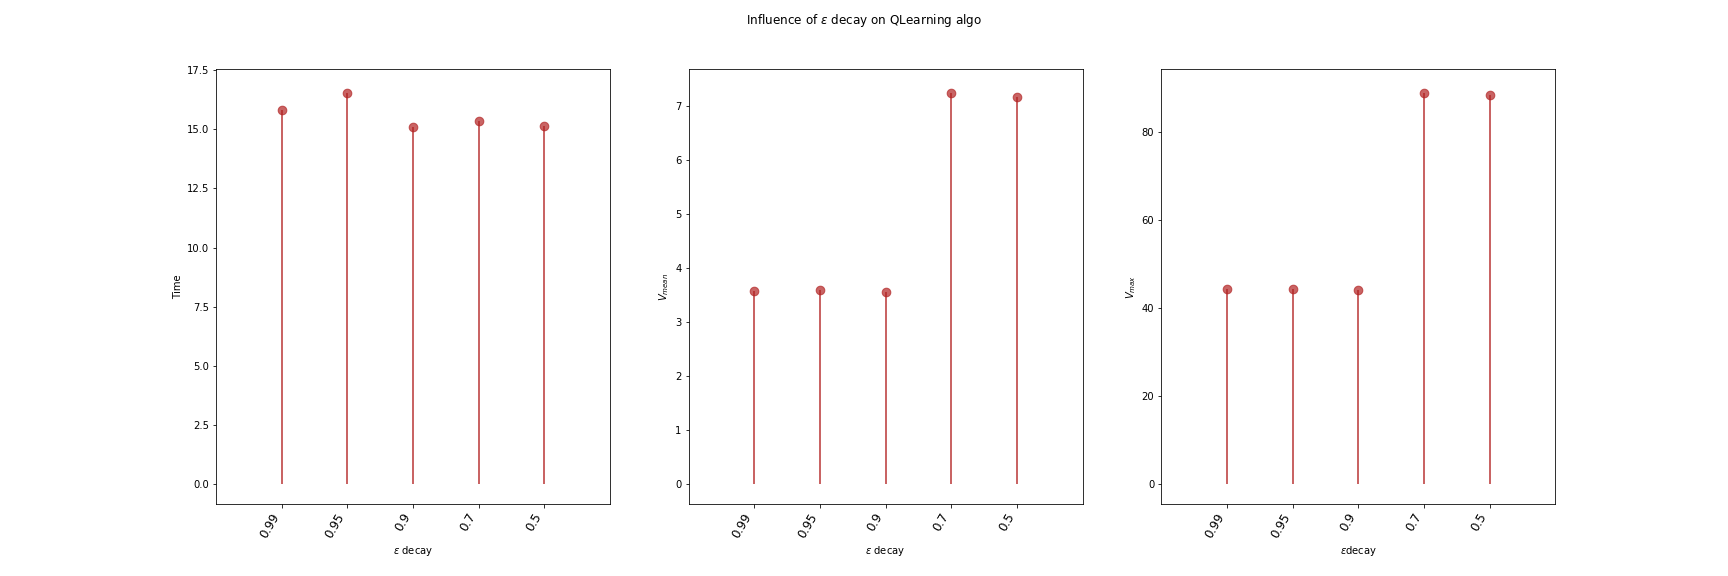
\includegraphics[width = \columnwidth]{epsdec_ql.png}
\caption{Influence of $\epsilon$ decay}
\end{figure}

\begin{figure}[H]
\centering
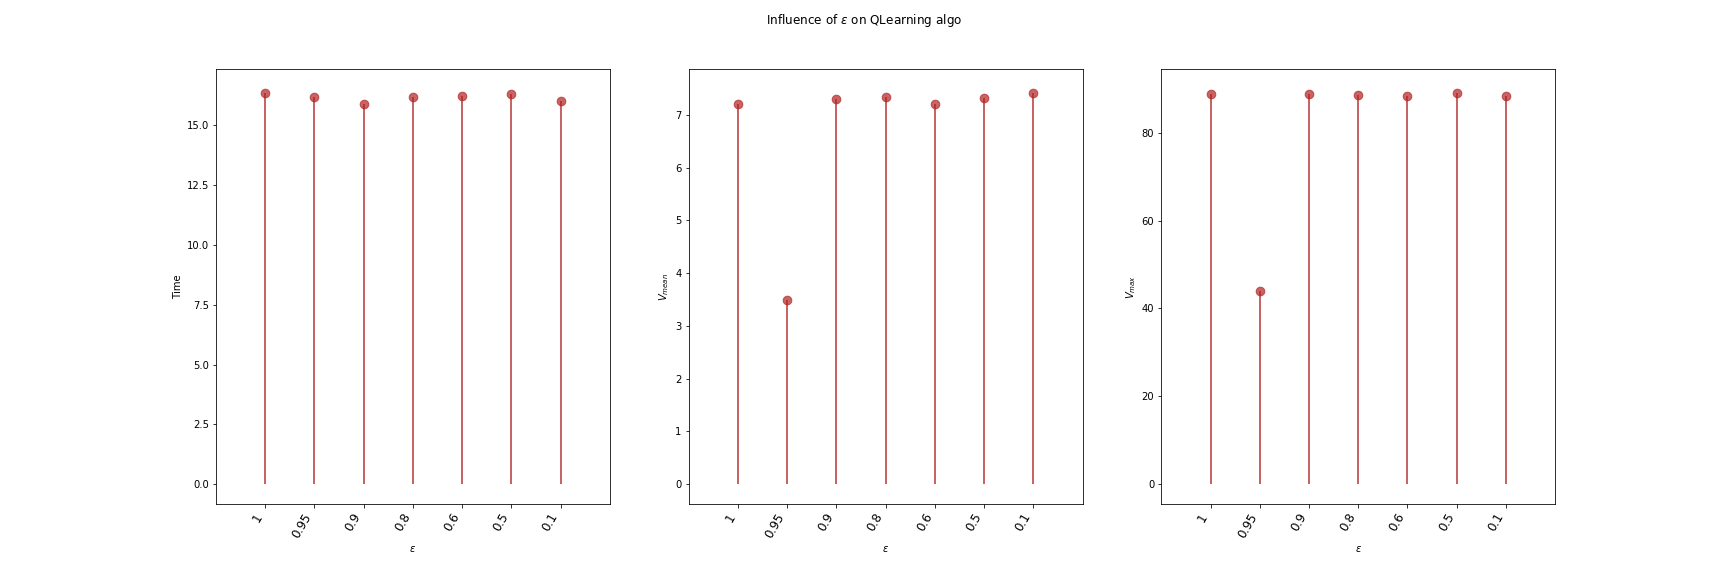
\includegraphics[width = \columnwidth]{eps_ql.png}
\caption{Influence of $\epsilon$}
\end{figure}

The results that I could obtain for the last graphs leave me a bit doubtful, there are few differences that are really noticeable and/or that I could explain. However, we can observe that changing a single hyperparameter can completely change the response of the algorithm. Below, we can observe three different answer with different values of $\epsilon$.

\begin{figure}[H]
\centering
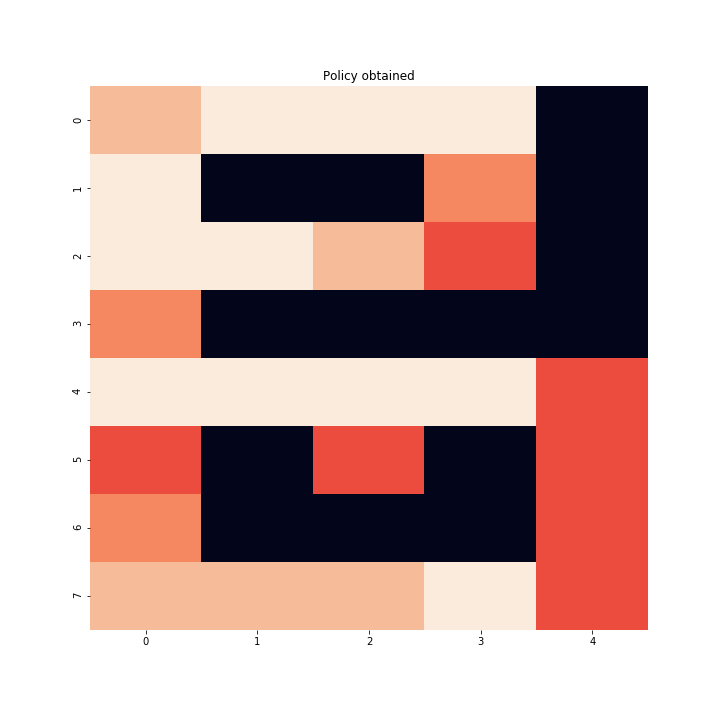
\includegraphics[scale = 0.3]{Policy_ql_eps7.png}
\end{figure}

\begin{figure}[H]
\centering
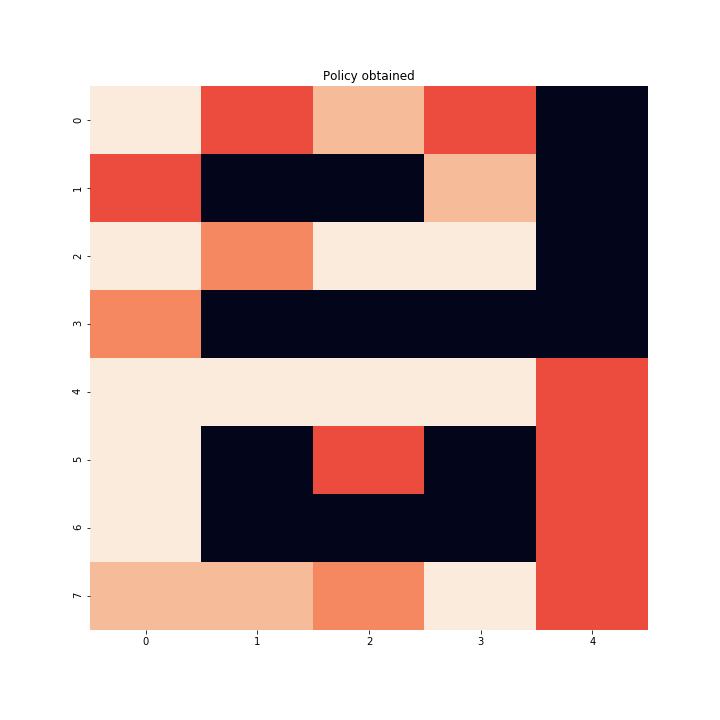
\includegraphics[scale = 0.3]{Policy_ql_eps4.png}
\end{figure}

\begin{figure}[H]
\centering
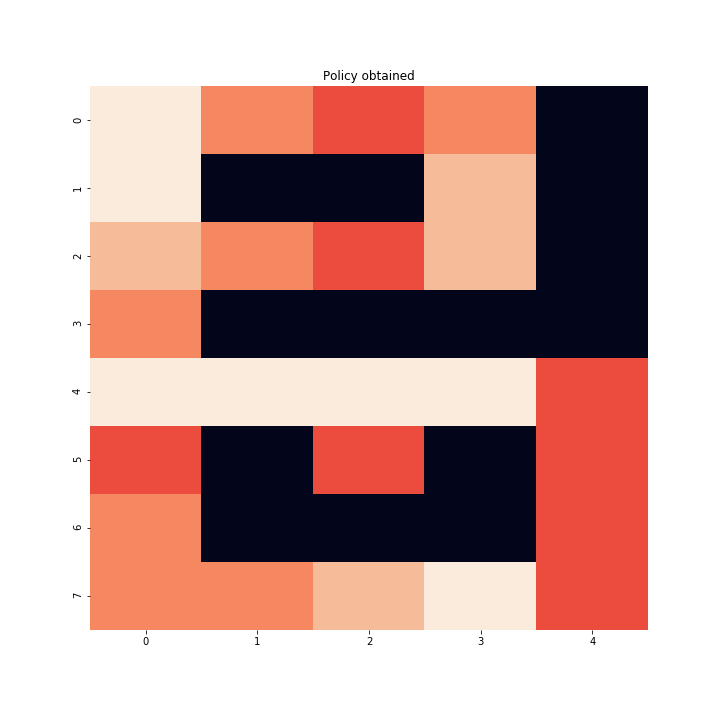
\includegraphics[scale = 0.3]{Policy_ql_eps2.png}
\end{figure}

In spite of these different answers (which do not correspond at all to the optimal policy - number of iterations not important enough), we can observe a remarkable fact. We find the idea of "information propagation" that we can note in the first algorithms like the Value Iteration. Indeed, even if the policy is not optimal because we have cut the process in progress, the states closest to the terminal states have already opted for the best policy. The information seems to propagate from the terminal states from one iteration to the next.

\section{Conclusion}

Through this assignment, we could see that most of the problems could be reduced in mathematical form to an optimization problem. Within the framework of MDPs, we have been able to study different algorithms to try to bring. The first two rely on the knowledge of the model to converge deterministically to an optimal answer using one of the variants of the Bellman equation. It should be noted that despite the apparent similarity in the convergence of these two methodologies towards the same policy, in most problems the use of Policy Iteration will be preferable. It requires less time and fewer iterations. However, some particular problems may allow Value Iteration to compete. For these first two algorithms, their performances are mainly due to the size of the problem and the choice on the notion of convergence and "vision of the future". The larger the problem, the more demanding the convergence, the longer the algorithm will take and the more iterations it will require.

Finally, the Reinforcement Learning (Q-Learning) algorithm is directly inspired by Simulated Annealing. It consists of a tradeoff between exploitation and exploration. It seems that the favorable strategy differs the problem. In the case of forest management, it would be mainly focused on exploitation and for the Grid World, it would be necessary to introduce more the notion of exploration. This type of reflection seems similar to the performance analysis on the SA. Indeed, for a function with few local optima, the quasi-pure exploitation is interesting (to reach quickly an answer with little chance to fall in a local optimum) whereas for a more complex function, we will ask more exploration to allow the algorithm to escape from a local optimum.

\end{multicols}

\end{document}